\subsection{Maximum Subarray:}

Demonstration that maximum subarray has complexity {\bfseries\itshape T ( n ) = ( n log n ) } order:  \hfill \break

{\bfseries\color{Violet}{function}} FIND-MAXIMUM-SUBARRAY (A, low, high)
\begin{lstlisting}[mathescape=true]
if high == low
	return (low, high, A[low])
else mid = [(low+high) / 2]
	(left_low, left_high, left_sum) = FIND-MAXIMUM-SUBARRAY(A, low, mid)
	(rigth_low, rigth_high, rigth_sum) = FIND-MAXIMUM-SUBARRAY(A, mid+1, high)
	(cross_low, cross_high, cross_sum) = FIND-MAX-CROSSING-SUBARRAY(A, low, mid, high)
	if left_sum $\leq$ right_sum and left_sum $\leq$ cross_sum
		return (left_low, left_high, left_sum)
	else if right_sum $\leq$ left_sum and right_sum $\leq$ cross_sum
		return (rigth_low, rigth_high, rigth_sum)
	else return (cross_low, cross_high, cross_sum)
\end{lstlisting} \hfill

\begin{itemize}
\item {\bfseries\itshape\color{Maroon}{Demonstration:}} 
\end{itemize} 

\begin{itemize}
\item {\bfseries\itshape\color{Violet}{First, our recurrence equations are:}}
\end{itemize} \hfill

\begin{ceqn}
\begin{align}
T( n ) = \left\{
\begin{array}{ll}
c & \mathrm {if\ } n = 1 \\
2T ( \frac{n}{2} ) + cn & \mathrm {if\ } n > 1 \\
\end{array}
\right.
\end{align}
\end{ceqn} \hfill

The next figure show how we can solve recurrence. For convenience, we assume that $n$ is an exact power of $2$.
The total number of levels of the recursion tree in the figure is $lg n + 1,$ where $n$ is the number of leaves, corresponding to the input size. An informal inductive argument justifies this claim. The base case occurs when $n = 1$, in which case the tree has only one level. Since $lg 1 = 0$, we have that $lg n + 1$ gives the correct number of levels. Now assume as an inductive hypothesis that the number of levels
of a recursion tree with $2^{i}$ leaves is $lg 2^{i} + 1 =  i + 1$ (since for any value of $i$, we have that $lg 2^{i} = i$). \hfill \break
To compute the total cost represented by the recurrence equation, we simply add up the costs of all the levels. The recursion tree has $lg n + 1$ levels, each costing $cn$,for a total cost of $cn(lg n + 1) = cn lg n + cn$. Ignoring the low-order term and the constant $c$ gives the desired result of $ \theta(n lg n)$.

\begin{figure}[H]
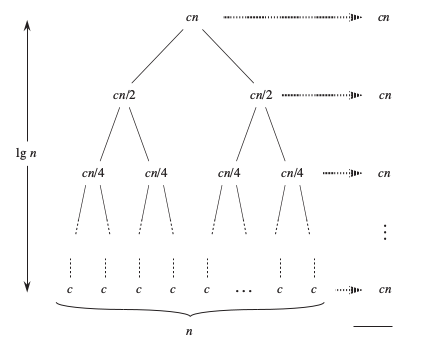
\includegraphics[scale=.6]{recurrence}
\centering \linebreak \linebreak Figure : Rcurrence Solve for Maximum Subarray.
\end{figure} 

\begin{itemize}
\item {\bfseries\itshape\color{Violet}{Finally:}}
\end{itemize} \hfill

\begin{ceqn}
\begin{align}
Maximum\  Subarray\ \in\ \theta\ (\ n\log\ n\ )
\end{align}
\end{ceqn}
\pagebreak